In this module you will learn
\begin{itemize}
	\item what is an autonomous differential equation
	\item how to obtain some properties of solutions of autonomous differential equations without solving them
\end{itemize}

\hfill \\




In this module, we focus on another type of differential equations.
The ultimate goal of this module is to learn that with some creativity and observation of the differential equation, it is possible to study solutions without actually solving them. \\


We start by defining autonomous equations.



\begin{definition}[Autonomous differential equations]
A first-oder DE is called \emph{autonomous} if it has the form
$$
y' = f(y).
$$
These are basically ODEs where the rate of change does not depend on time, meaning that the nature of the ODE always stays the same.

%The zeros of the function $f$ are called \emph{critical points}. They can also be called \emph{equilibrium} or \emph{stationary} points.
\end{definition}


\begin{graybox}
Observe that autonomous ODEs are also Separable ODEs.	
\end{graybox}


So let us look at an autonomous ODE and think what happens when $f(y_0)=0$?

Then if the solution is unique (what are the conditions that will guarantee that?) and if $y(t_0)=y_0$, that means that
$$
y'(t_0) = f(y_0)=0.
$$

So we can find one immediate solution:
$$
y(t) = y_0,
$$
a constant solution. Since the solution is unique, that must be \textbf{the} solution. \\


This is a property of autonomous ODEs:

\begin{definition}[Equilibrium points]
Consider an autonomous ODE $y'=f(y)$.
The zeros of the function $f$ are called \emph{critical points}. They can also be called \emph{equilibrium} or \emph{stationary} points.
\end{definition}

\begin{important}
Consider an autonomous ODE $y'=f(y)$ and let $c$ be a zero of $f$, i.e. $f(c)=0$.

Then the constant function $y(t) = c$ is a solution of the ODE, called an \emph{equilibrium solution}.
\end{important}


In an ODE where solutions are unique, these equilibrium solutions are extremely important, as they give bounds for all other solutions.


\begin{example}
Consider the autonomous ODE
$$
y'=\sin(2y).
$$

The \emph{equilibrium solutions} for this ODE are
$$
y = k\pi,
$$
for all values $k \in \mathbb{Z}$.

That means that even without solving, we can infer that the solution passing through $y(0)=1$, must satisfy
$$
y(t) \in (0,\pi),
$$
for all $t$.	
\end{example}


Equilibrium solutions are even more important, because we can also study what happens between equilibrium solutions without having to actually solve the ODE.

If the function $f(y)$ is continuous, then its sign cannot change between equilibrium points, so the solutions will be monotonic between equilibrium solutions.

\begin{example}
Consider the same ODE:
$$
y'=\sin(2y).
$$

We can study whether solutions will be increasing or decreasing by studying the function $f(y)$.

\begin{center}
\begin{tabular}{c|ccccccccccc}
$y$ & $\cdots$ & $-2\pi$ & & $-\pi$ & & $0$ & & $\pi$ & & $2\pi$ & $\cdots$ \\[5pt]%\hline
$y'=\sin(2y)$ & & $0$ & $+$ & $0$ & $-$ & $0$ & $+$ & $0$ & $-$ & $0$ & \\[5pt]\hline\hline
$y(t)$ & $\cdots$ & $c$ & $\nearrow$ & $c$ & $\searrow$ & $c$ & $\nearrow$ & $c$ & $\searrow$ & $c$ & $\cdots$
\end{tabular}	
\end{center}

In a graph, we have
\begin{center}
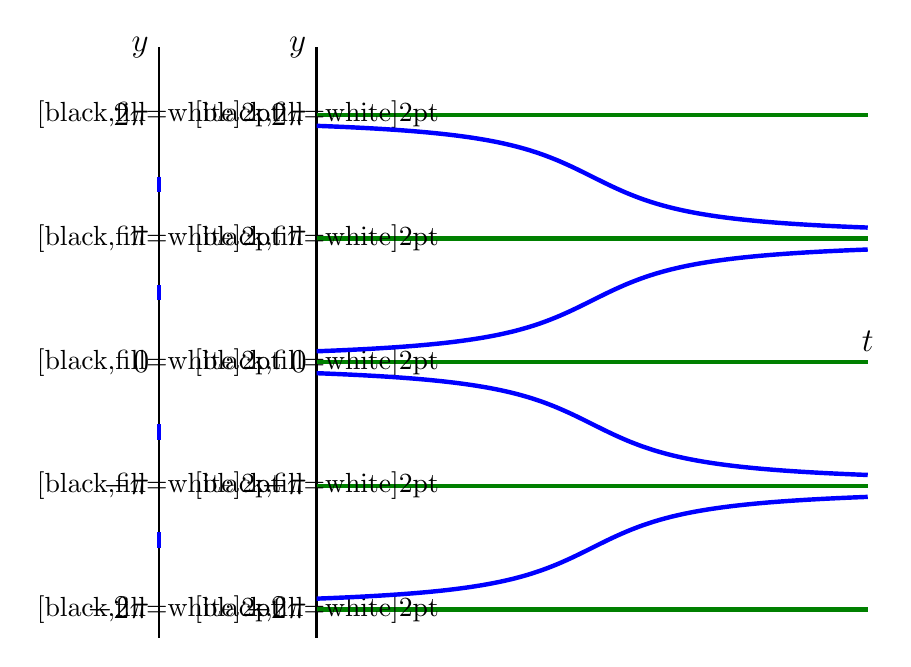
\begin{tikzpicture}
  \draw[thick] (-2,-3.5) -- (-2,4) node[left] {\large $y$};
  \draw[thick,-{\seta}] (0,0) -- (7,0) node[above] {\large $t$};
  \draw[thick,-{\seta}] (0,-3.5) -- (0,4) node[left] {\large $y$};
  \foreach \k in {-2,...,2} {
    \draw[ultra thick, green!50!black] (0,{\k*pi/2}) -- (7,{\k*pi/2});
    \draw (-2,{\k*pi/2}) node {\tikzcircle[black,fill=white]{2pt}};
    \draw (0,{\k*pi/2}) node {\tikzcircle[black,fill=white]{2pt}};
  }
  \foreach \k in {-2,0} {
    \draw ({\k},0)  node[left] {\large $0$};
    \draw ({\k},{pi/2})  node[left] {\large $\pi$};
    \draw ({\k},{pi})  node[left] {\large $2\pi$};
    \draw ({\k},{-pi/2})  node[left] {\large $-\pi$};
    \draw ({\k},{-pi})  node[left] {\large $-2\pi$};
    \draw[samples=40, ultra thick,domain=0:7,smooth,variable=\x,blue] plot ({\x},{rad(atan(\x-3.5))/2+pi/4+\k*pi/2});
    \draw[samples=40, ultra thick,domain=0:7,smooth,variable=\x,blue] plot ({\x},{-rad(atan(\x-3.5))/2+3*pi/4+\k*pi/2});
    \draw[ultra thick,-{\seta},blue] (-2,{pi/4+\k*pi/2}) -- (-2,{pi/4+0.2+\k*pi/2});
    \draw[ultra thick,-{\seta},blue] (-2,{-pi/4-\k*pi/2}) -- (-2,{-pi/4-0.2-\k*pi/2});
  }
\end{tikzpicture}
%	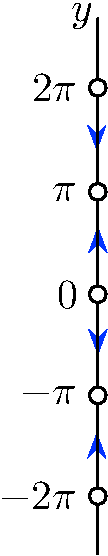
\includegraphics[height=150pt]{images/module14-equil1.pdf}
%	\quad 
%	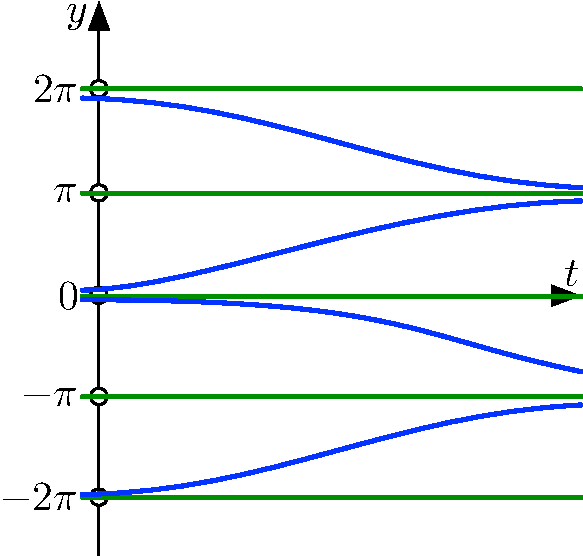
\includegraphics[height=150pt]{images/module14-equil2.pdf}
\end{center}

We can infer that the graphs will approach the constant solutions without touching because the derivative $y'$ will become smaller and smaller the more they approach the equilibria. We also know that solutions cannot touch each other.
\end{example}

There is also a distinction that we make about equilibrium points that helps us understand the behaviour of solutions. We will study this distinction in the core exercises.







\paragraph{\color{cyan}Population Models.} The fact that these differential equations keep the same rate of change independently of time, makes them an ideal candidate when studying populations.

%
%
%
%
%
%
%
%\paragraph{Exponential Growth. } 
%
%
%$P(t) = $ size of a certain population at time $t$
%
%\paragraph{Malthusian Population Model:}
%The population increases/decreases proportionally to its size, i.e.,
%$$
%\frac{dP}{dt} = rP,
%$$
%for some growth rate $r$.
%
%The solution of this DE is
%%    
%%    This is a separable $DE$, so we can solve it:
%%    \begin{align*}
%%    \frac{1}{P} \frac{dP}{dt} & = k \\
%%    \int \frac{1}{P} dP & = \int k dt \\
%%    \ln|P| &= kt + C \\
%%    |P| & = e^{kT+C} = e^C e^{kt} = A e^{kt}
%%    \end{align*}
%%    for $A = e^C >0$.
%%    
%%    So
%\[\tag{Review Exercise}
%P = P(0) e^{rt}.
%\]
%
%\begin{itemize}
%\item Population grows exponentially if $r>0$;
%\item Population decays exponentially if $r<0$.
%\end{itemize}
%
%This method is good while the environment can provide for all the population. Since there are no infinite environments, this method will ultimately fail! 
%
%
%\paragraph{Logistic Model:} Modification of the Malthusian model, to model an environment with limited resources. The individuals in the population are competing for resources among themselves:
%$$
%\frac{dP}{dt} = rP - \alpha P^2,
%$$
%where $P^2$ gives the number of possible encounters between individuals, and $\alpha$ gives a constant on how competition decreases the growth. 
%
%Another way to obtain this model is by observing that the rate of growth decreases as the population increases, so the simplest way to substitute $r$ with $r-\alpha P$ not the Malthusian Model. We obtain
%$$
%\frac{dP}{dt} = (r-\alpha P) P.
%$$
%
%Usually we write $\alpha = \frac rK$, so the model is
%\[\tag{Logistic Growth}
%\frac{dP}{dt} = r P \left(1 - \frac{P}{K}\right),
%\]
%for some intrinsic growth rate $r>0$ (the growth rate without limiting factors).
%
%This equation has two equilibrium solutions:
%$$
%P(t) = 0 \qquad \text{ and } \qquad P(t) = K.
%$$
%
%
%From the equation we observe the following: \\
%
%\begin{minipage}{10cm}
%\begin{itemize}
%\item The solutions cannot cross the line $y=K$: if they did, at $y=K$ they would have $y'=0$ and would remain at $y=K$
%
%\item Look the function $f(P) = \frac rK y(K-y)$ and analyze its sign:
%
%\item if $0<y(0)<K$, then $y' = f(y) > 0$, so the solution will keep increasing
%\item if $y(0)>K$, then $y' = f(y) < 0$, so the solution will keep decreasing
%
%\end{itemize}
%\end{minipage}
%\hfill
%\begin{minipage}{175pt}
%\includegraphics*[width=175pt]{figures/0205_auton.pdf}
%\end{minipage}
%
%\hfill\\
%
%We can now classify the equilibrium solutions:
%\begin{itemize}
%\item $P=0$ is unstable
%\item $P=K$ is stable
%\end{itemize}
%
%
%We can then conclude that the solutions will look like:
%\begin{center}
%\includegraphics*[width=150pt]{figures/0205_logpop.pdf}
%\end{center}
%
%\begin{rem}
%And the constant $K$ is the maximum number of individuals that the environment can sustain.
%\end{rem}
%
%
%We can solve this separable equation to obtain
%%
%%
%%\begin{gather*}
%%\frac{dP}{dt} = \frac rK P \left(K-P\right) \\
%%\frac{1}{P(K-P)} \frac{dP}{dt} = \frac rK \\
%%\\
%%\frac{1}{P(K-P)} = \frac AP + \frac{B}{K-P} \\
%%1 = A(K-P) + BP\\
%%AK=1\\
%%BK=1\\
%%\\
%%\left( \frac{1}{P} + \frac{1}{K-P}\right) \frac{dP}{dt} = r \\
%%\\
%%\ln|P| - \ln|K-P| = r t +C\\
%%\frac{P}{K-P} = c e^{rt} \\
%$$
%P(t) = \frac{K}{1+ce^{-rt}} 
%$$
%%\end{gather*}
%
%
%%
%%
%%To simplify the notation, we relabel the equation to
%%$$
%%\frac{dP}{dt} = P \left(a-bP\right),
%%$$
%%for $a,b>0$.
%%
%%
%%
%%This DE is separable, so we can solve it:
%%\begin{align*}
%%\frac{1}{P(a-bP)} \frac{dP}{dt} & = 1 \\
%%\int \frac{1}{P(a-bP)} dP & = \int 1 dt = t+C.
%%\end{align*}
%%
%%Using partial fractions, we write
%%\begin{align*}
%%\frac{1}{P(a-bP)}
%%	& = \frac{A}{P} + \frac{B}{a-bP} \\
%%	& = \frac{ A(a-bP) + BP}{P (a-bP)} \\
%%	& = \frac{ Aa + (B-Ab)P}{P (a-bP)}.
%%\end{align*}
%%
%%So $Aa = 1$ and $B-Ab = 0$. We have
%%$$
%%A = \frac{1}{a} \qquad \text{ and } \qquad B = \frac{b}{a}.
%%$$
%%
%%We now have
%%$$
%%\int \frac{1}{P(a-bP)} dP
%%	 = \int \frac{1}{a} \left(\frac{1}{P} + \frac{b}{a-bP}\right) dP
%%	 = \frac{1}{a} \left( \ln |P| - \ln |a-bP| \right)
%%	 = \frac{1}{a} \ln \left| \frac{P}{a-bP}\right|
%%$$
%%
%%The solution of the DE is given by
%%\begin{align*}
%%\frac{1}{a} \ln \left| \frac{P}{a-bP}\right| & = t+C \\
%%\ln \left| \frac{P}{a-bP}\right| & = at+aC \\
%%\left| \frac{P}{a-bP}\right| & = e^{aC}e^{at} = C_1 e^{at}
%%\end{align*}
%%for $C_1=e^{aC}>0$.
%%
%%We have
%%$$
%%\frac{P}{a-bP} =  \pm C_1 e^{at} = C_2 e^{at}.
%%$$
%%
%%Now we solve for $P$:
%%\begin{align*} 
%%P & = C_2 e^{at} (a-bP) \\
%%\left( 1 +C_2 b e^{at} \right) P & = C_2 a e^{at} \\
%%P & = \frac{C_2 a e^{at}}{1 +C_2 b e^{at}} \\
%%P & = \frac{a}{b + \frac{1}{C_2} e^{-at}}
%%\end{align*}
%%
%%We know that $\ds C_2 = \frac{P(0)}{a-bP(0)}$, so
%%$$
%%P(t) = \frac{a}{b + \left(\frac{a}{P(0)}-b\right) e^{-at}} 
%%= \frac{K}{1 + \left(\frac{K}{P(0)}-1\right) e^{-rt}}.
%%$$
%%
%%We can verify that $P(t) \to K$ as $t \to \infty$.
%\begin{note}
%We can improve on these models. For example, we can include a threshold of survivability, where if a population goes below that level, it will eventually become extinct.
%
%\subparagraph{Exercise. } Study the model
%$$
%\frac{dP}{dt} = -r\left(1-\frac PT\right) \left(1-\frac PK\right) P,
%$$
%where $r>0$ and $0<T<K$.
%\end{note}
%
%
%
%\paragraph{``Jelly Fish'' from MAT187. } 
%
%
%On a question of a midterm on MAT187, we studied another DE for a ``jelly fish'' population:
%$$
%\frac{dP}{dt} = r(P-T)(P-K)^2,
%$$
%for $0<T<K$.
%
%We can quickly study this problem qualitatively by studying the function: $f(y) =  r(y-T)(y-K)^2$.
%
%The equilibrium points are:
%$$
%T \quad , \quad K\quad .
%$$
%We study the sign of $f(y)$:
%
%\begin{center}
%\includegraphics*[width=200pt]{figures/0202_jellyfish.pdf}
%\hfil
%\includegraphics*[width=150pt]{figures/0202_jellyfish_sols.pdf}
%\end{center}
%
%We can also classify the equilibrium solutions:
%\begin{itemize}
%\item $P=T$ is unstable
%\item $P=K$ is semi-stable (stable from below and unstable from above)
%\end{itemize}
%
%
%And we can analyze the solutions:
%\begin{itemize}
%\item If $0< P_0 < T$, then the population will go extinct (in finite time). It doesn't just approach extinction asymptotically, it really does go extinct, as the slope keeps increasing (with negative sign)
%
%\item If $T<P<K$, then the population thrives and increases its number approaching $P=K$.
%
%\item If $T>K$, then the population increases at an accelerating pace. It goes ``viral''!
%\end{itemize}
%
%
%
%\subparagraph{Exercise. } Read Pages 81--83: Critical points and stable/unstable equilibrium solutions.



\begin{video}
\begin{itemize}
	\item \qrvideo{https://youtu.be/swt-let4pCI} %\href{https://youtu.be/swt-let4pCI}{https://youtu.be/swt-let4pCI} \hfill \qrcode{https://youtu.be/swt-let4pCI}
\end{itemize}	
\end{video}



